\skriptsection{Filtering in the Frequency Domain (V4)}{199}

\subsection{Discrete Fourier Transform (DFT)}
\begin{minipage}{11cm}
  \skriptsubsubsection{1-Dimensional}{220}
   $$s(h)=\sum_{k=0}^{N-1}\hat c_k e^{jhk\frac{2\pi}{N}}=
     \sum_{k=0}^{N-1} \left[ \hat{a}_k \cos\left(hk \frac{2 \pi}{N}\right)+\hat{b}_k \sin\left(hk
    \frac{2 \pi}{N}\right) \right]$$ with $N$ as the periodic number and the coefficients:\\
    $\hat{c}_k=\frac{1}{N} \sum\limits_{h=0}^{N-1}s(h) e^{-jhk\frac{2\pi}{N}}=\hat{a}_k-j\hat{b}_k = \Re\{c_k\} + j \Im\{c_k\}$ \\
    $\hat{a}_k=\frac{1}{N} \sum\limits_{h=0}^{N-1}s(h) \cos\left(hk \frac{2 \pi}{N}\right)=\Re\{\hat{c}_k\}$ \\
    $\hat{b}_k=\frac{1}{N} \sum\limits_{h=0}^{N-1}s(h) \sin\left(hk \frac{2 \pi}{N}\right)=-\Im\{\hat{c}_k\}$ 
  
  \skriptsubsubsection{2-Dimensional}{225}
    $$F(u,v) = \frac{1}{\sqrt{M N}} \sum_{x=0}^{N-1} \sum_{y=0}^{M-1} f(x,y) \exp\left( -j 2 \pi \left(\frac{ux}{M} + \frac{v y}{N} \right) \right)$$
\end{minipage}
\begin{minipage}{8cm}
  Beware, the Fast Fourier Transform is exactly the same as the DFT but faster.
  The phase contains important information and should not be discarded.\\
  
  To find out amplitude and phase:\\
  $|F(u,v)| = \sqrt{\Re\{F(u,v)\}^2 + \Im \{F(u,v)\}^2}$,\\
  $\varphi(u,v) = \arctan\left( \frac{\Im \{F(u,v)\}}{\Re\{F(u,v)\}} \right)$\\
  
  Examples of 2D-Fourier transform pairs \gonzales{243}.\\
  Fourier transform properties \gonzales{253f.}.\\
  
  In 2D, the DC values are visible at coordinates (0,0), but to better visualize the spectrum they 
  are usually moved to the center \matlab{fftshift}.  
\end{minipage}

\begin{minipage}{8cm}

\subsection{Border Problems}
  Due to the periodicity of the Fourier transform, borders are reproduced when no measures are taken.
  
  $F(k+N) = \sum\limits_{n=0}^{N-1} x_n e^{-\frac{2\pi j}{N} (k+N) n}$\\
  $=\sum\limits_{n=0}^{N-1} x_n e^{-\frac{2\pi j}{N} k n}  \underbrace{e^{-2 \pi j n}}_{1} = 
    \sum\limits_{n=0}^{N-1} x_n e^{-\frac{2\pi j}{N} k n} = F(k)$

\subsubsection{Padding}
  One way to avoid border problems is padding the original input image.
  
  From p. 263:
  \begin{aufzaehlung}
    \item Obtain padding parameters from input image $f(x,y)$ of size $M$x$N$. The padding parameters are 
    $P = 2M$ and $Q = 2N$
    \item Append zeros to input image to obtain the padded image $f_p(x,y)$
    \item Center its transform:\\
      $f_c(x,y) = f_p(x,y) \cdot (-1)^{x+y}$
    \item Compute DFT:\\
      $f_c(x,y) \FT F(u,v)$
    \item Filter:\\
      $F_f = F(u,v) \cdot H(u,v)$
    \item Compute IDFT:\\
      $F(u,v) \IFT g_p(x,y)$
    \item Extract original region $M$x$N$ from $g_p(x,y)$
  \end{aufzaehlung}
\end{minipage}
\begin{minipage}{11cm}
  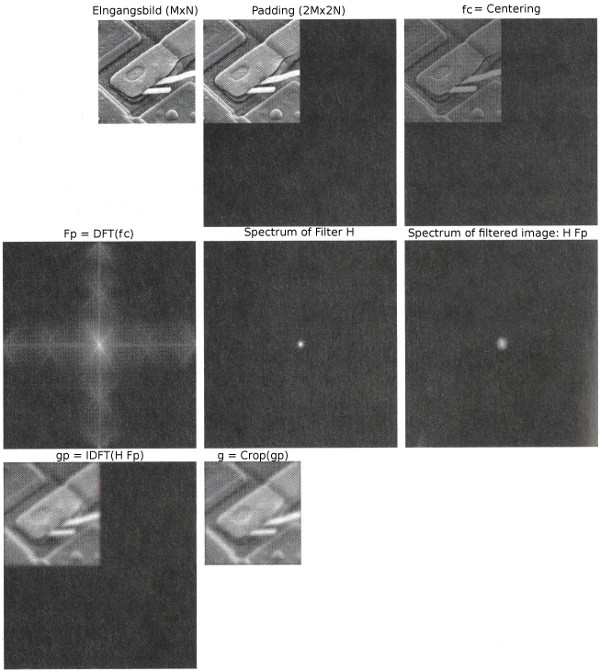
\includegraphics[width=11cm]{./images/frequency_filtering_padding.jpg}
\end{minipage}

\clearpage
\subsubsection{Window}
Another way is use windowing function which have nearly the size of the image and which smooth at 
the border to zero. In the spatial domain, they can be multiplied (which leads to convolution in 
the frequency domain).

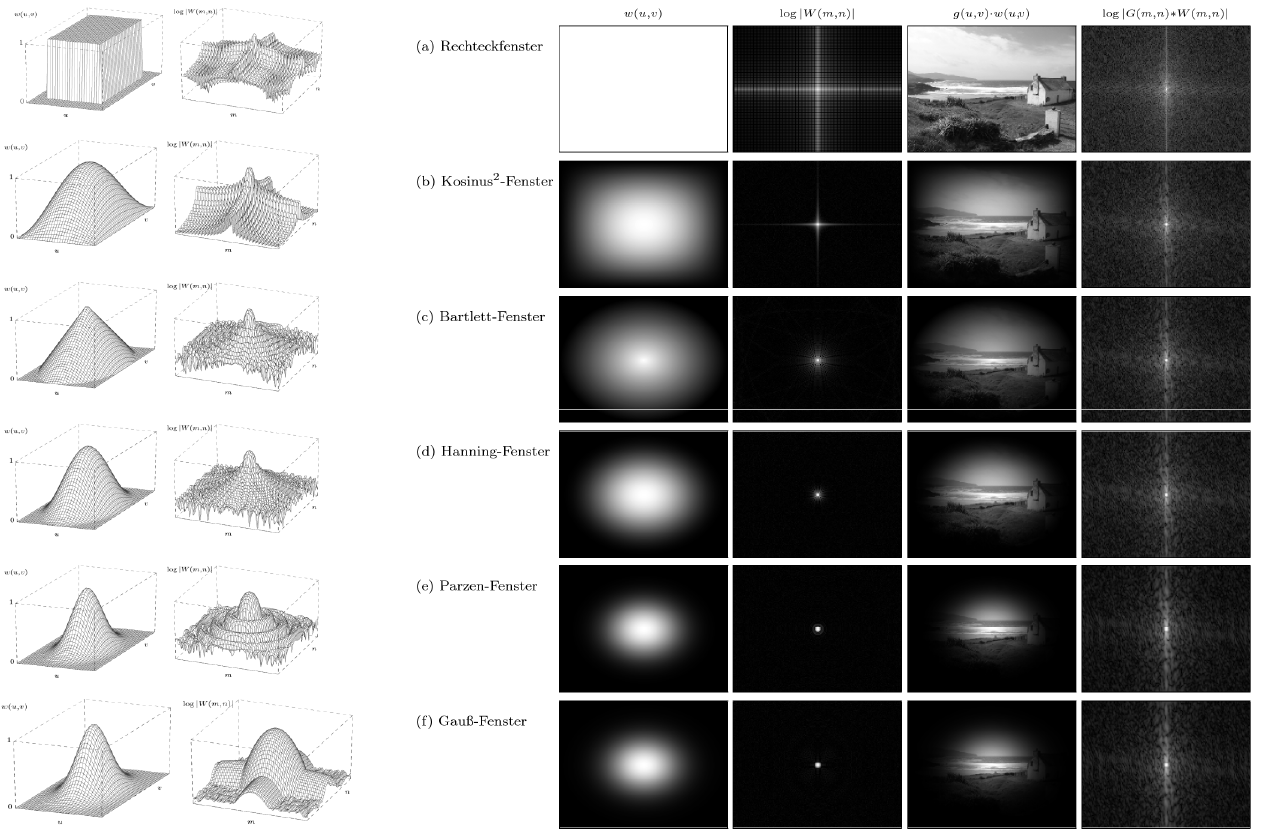
\includegraphics[width=\linewidth]{./images/window_functions.png}

\skriptsubsection{Filter Types}{269}
Filtering periodic noise can easily be done in the frequency domain.
E.g. band-rejection (notch) filter.\\
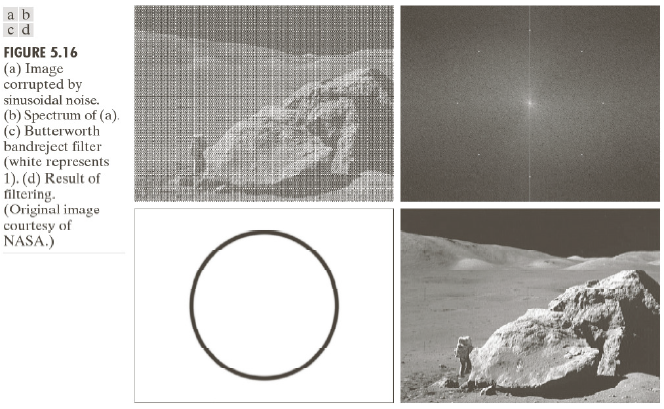
\includegraphics[width=10cm]{./images/periodic_noise_filter.png}